\documentclass{article} % kind of document 
\usepackage[utf8]{inputenc} %encoding of choice
\usepackage[american]{babel} %language of choice
\usepackage[p,osf]{cochineal}
\usepackage{fancyhdr} %for header
\usepackage{amsmath, tabu} %math mode
\usepackage{mathtools}
\usepackage{amssymb} %math symbols
\usepackage{dsfont} %specifically for the indicator function symbol
\usepackage{xcolor} %to color text
\usepackage{amsthm} %math theorem
\usepackage{tikz}
\usepackage{caption}
\usepackage{multirow}
\usepackage[bottom]{footmisc}
% \usepackage[dvipsnames]{xcolor}
\usepackage{enumerate} %make lists
\usepackage{graphicx} %insert images
\usepackage{float} %to fix image position
\usepackage{moreverb} %to make boxes
\usepackage{hyperref} %to create hyperlinks
\usepackage{lipsum} %lorem ipsum package
\usepackage{setspace} % to use singlespace below in the solution environment
\usepackage[shortlabels]{enumitem}
\usepackage{parskip}
\usepackage[us]{datetime} %package for setting due date in US format
\newdate{duedate}{27}{04}{2021} %to set a due date
\usepackage{jlcode}
\allowdisplaybreaks
\usepackage[margin=1in]{geometry}
\pagestyle{fancy}


\lhead{Due: \displaydate{duedate}}
\chead{ECON 899 -- Problem Set 2 }
\rhead{}


\DeclareMathOperator*{\E}{\mathbb{E}} %ease of writing e and E
\newcommand{\e}{\mathrm{e}}
\newcommand{\ct}{\mathsf{c}}
\newcommand{\Z}{\mathbb{Z}}
\newcommand{\R}{\mathbb{R}}
\newcommand{\N}{\mathbb{N}}
\newcommand{\ifn}{\mathds{1}}
\newcommand{\X}{\mathbf{X}}
\newcommand{\Y}{\mathbf{Y}}
\newcommand{\one}{\mathbf{1}}
\newcommand\numberthis{\addtocounter{equation}{1}\tag{\theequation}}
\newcommand*\widebar[1]{\overline{#1}} % to get a widebar
\theoremstyle{definition}
\newtheorem{theorem}{theorem} % Theorem display format
\newtheorem{problem}[theorem]{Exercise} % Problem display format, last bracket sets display choice

\newenvironment{solution}[1][Answer]{\begin{singlespace}\underline{\textbf{#1:}}\quad }{\ \rule{0.3em}{0.3em}\end{singlespace}} % Answer format

\newenvironment{solutions}[1][Proof]{\begin{singlespace}\underline{\textbf{#1:}}\quad }{\ \rule{0.3em}{0.3em}\end{singlespace}} % Answer format

\begin{document}

This problem set was completed by Danny Edgel, Mitchell Valdes Bobes, Ryan Mather, and Yobin Timilsena.
	\begin{enumerate}[I.]
		\item Consider the same environment as Huggett (1993, JEDC) except assume that there are enforceable insurance markets regarding the idiosyncratic shocks to earnings and that there are no initial asset holdings. Solve for a competitive equilibrium. What are prices? What is the allocation? (Hint: think about the planner’s problem and then decentralize).
		\begin{solution}
			Under the assumptions of enforceable insurance markets + locally non-satiated preferences, the basic first and second welfare theorems hold. Hence, we will solve the planner's problem for allocations and then decentralize by setting asset prices that support the allocations as a CE.
			
			The planner's problem can be written as
			\begin{align*}
				\E_0 \sum_{t=0}^\infty \beta^t [ \pi(e) u(c_{e,t}) + \pi(u) u(c_{u,t}) ] \;\; \text{ s.t. } \;\; \pi(e) c_{e,t} + \pi(u) c_{u,t} \leq \pi(e) y_t(e) + \pi(u)y_t(u), \; \forall t
			\end{align*}
			The first order conditions are
			\begin{align*}
				[c_{e,t}]:   \beta^t \pi(e) u'(c_{e,t})  = \lambda \pi(e)   &&     [c_{u,t}]:  \beta^t \pi(u) u'(c_{u,t})  = \lambda \pi(u) 
			\end{align*}
		Combined, we have that $ u'(c_{e,t}) = u'(c_{u,t}) \Leftrightarrow c_{e,t} = c_{u,t} = \bar{c}$. 
		
		Plugging into the BC, we get $ \bar{c} = y_t(u) + \pi(e)[y_t(e) - y_t(u)] $. For instance, in Part II, we are given $ \pi(e) = 0.94 $, $ y_t(e) = 1 $ and $ y_t(u) = 0.5$, which would imply $ \bar{c} = 0.97$.
		
		The decentralized EE for an individual $ i $ is $ \beta^t u'(c_t^i)  = \lambda q_t \Leftrightarrow q_{t+1} = \beta q_t = \beta^{t+1} q_0$. 
		\end{solution}
	
		\item  Now compute Huggett (1993, JEDC) with incomplete markets. The following takes you through the steps of solving a simple general equilibrium model that generates an endogenous steady state wealth distribution. The basic algorithm is to: 1) taking a price of discount bonds $ q \in [0,1] $ as given , solve the agent's dynamic programming problem for her decision rule $ a' = g_\theta (a,s;q) $ where $ a \in A $ are asset holdings, $s \in S  \subset R_{++} $ is exogenous earnings, and $ \theta $ is a parameter vector; 2) given the decision rule and stochastic process for earnings, solve for the invariant wealth distribution $ \mu^* (A, S; q) $; 3) given $ \mu^* $, check whether the asset market clears at $ q $ (i.e. $\int_{A,S} g_\theta (a,s;q) \mu^*(da,ds;q) = 0$). If it is, we are done. If not (i.e. it is not within an acceptable tolerance), then bisect $[0,1]$ in the direction that clears the market (e.g. if $ \int_{A,S} a' \mu^* (da,ds;q) > 0 $), then choose a new price $ \hat{q} = q + [1 - q]/2 $ and go to step 1.
		
		\begin{enumerate}[4.]
			\item After finding fixed points of the $ T $ and $ T^* $ operators, answer the following questions:
			\begin{enumerate}[a.]
				\item  Plot the policy function $ g(a, s) $ over $ a $ for each $ s $ to verify that there exist $ \hat{a} $ where
				$ g(\hat{a}, s) < \hat{a} $ as in Figure 1 of Huggett. (Recall this condition establishes an upper bound on
				the set $ A $ necessary to obtain an invariant distribution).
				\begin{solution}
					The policy function is graphed below in Figure \ref{4a}. As can be seen, there does exist an $\hat{a}$ beyond which modeled agents always, whether employed or unemployed, dissave on net. 
					\begin{figure}[htbp!]
					\centering
					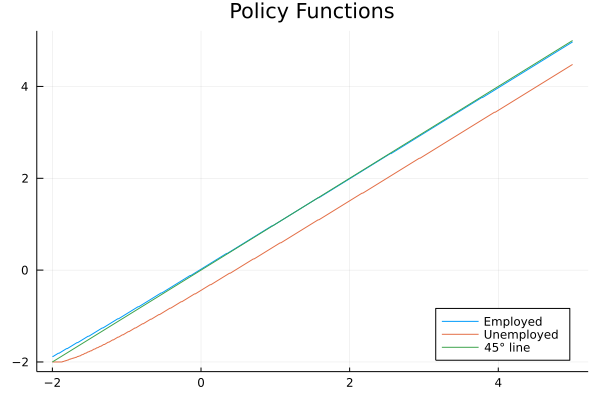
\includegraphics[scale=.5]{ForIncludingInDocument/02_ryan_Policy_Functions.png}
					\caption{Problem 4(a) \label{4a}}
					\end{figure}
				\end{solution}
			
				\item What is the equilibrium bond price? Plot the cross-sectional distribution of wealth for those employed and those unemployed on the same graph.
				\begin{solution}
					
				\end{solution}
			
				\item Plot a Lorenz curve. What is the gini index for your economy? Compare them to the data. For this problem set, define wealth as current earnings (think of this as direct deposited
				into your bank, so it is your cash holdings) plus net assets. Since market clearing implies aggregate assets equal zero, this wealth definition avoids division by zero in computing the Gini and Lorenz curve.
				\begin{solution}
					
				\end{solution}
			\end{enumerate}
		\end{enumerate}
		
		\item 
		\begin{enumerate}
			\item Plot $ \lambda(a,s) $ across $ a $ for both $ s = e $ and $ s = u $ in the same graph. 
			\begin{solution}
				
			\end{solution}
			\item What is $ W^{FB} $? What is $ W^{INC}  = \sum_{(a,s) \in A \times S} \mu(a,s) \nu(a,s) $? What is WG?
			\begin{solution}
				
			\end{solution}
			\item What fraction of the population would favor changing to complete markets? That is $   \sum_{(a,s) \in A \times S}   \ifn_{\lambda(a,s) \geq 0}  (a,s) \mu(a,s) $.
			\begin{solution}
				
			\end{solution}
		\end{enumerate}
	\end{enumerate}
\section*{Code Appendix}
This is the ``computation'' code that does most of the numerical work involved for the solutions above:
\jlinputlisting{./ForIncludingInDocument/Compute_Draft1.jl}

This code calls the ``computation'' code above and then prints some figures:
\jlinputlisting{./ForIncludingInDocument/RunCode_Draft1.jl}


\end{document}